\chapter{Kinship} \label{chap:kinship}

\section{Introduction}
\is{kinship!abbreviation}
Kinship terms (§\ref{sec:kinship}) in Japhug are all inalienably possessed nouns (§\ref{sec:inalienably.possessed}), and are presented in this section in their indefinite possessor form (§\ref{sec:indef.genr.poss}), which generally also serves as the citation form.

This section is not concerned with the morphosyntactic properties of these nouns (which is treated in §\ref{sec:indef.genr.poss}), but rather with the semantic structure of the system. 

The meanings of the terms are described using the abbreviations presented in \tabref{tab:kinship.abb}, which, combined with each other (for instance MB and  eZ represent `mother's brother' and  `elder sister', respectively), offer a concise way to represent the possible parameters relevant to the description of kinship terms \citep{kroeber1909classificatory}. 

 
\begin{table}
\caption{Standard abbreviations used to describe kinship terms} \label{tab:kinship.abb}
\begin{tabular}{llXllXlll}
\lsptoprule
F & Father & M & Mother \\
B & Brother & Z & Sister \\
S & Son & D & Daughter & Ch & Child \\
H & Husband & W & Wife \\
♂  & Male possessor & ♀& Female possessor \\
e/+ & Elder & y/- & Younger \\
\lspbottomrule
\end{tabular}
\end{table}

The term ``male/female possessor'' corresponds to what \citet[78--79]{kroeber1909classificatory} calls `sex of the person through whom the relationship exists' or `sex of the connecting relative', encoded as inalienable possessor in Japhug. For instance, \japhug{tɤ-snom}{sister} (\textsuperscript{♂}Z) is only used with reference to the sister of a male (§\ref{sec:siblings.gender}).

Kinship terms can be divided into self-reciprocal terms, in which both members of the relationship use the same term to refer to each other (from instance \japhug{tɤ-mɤtsa}{mother's sister's child} MZCh, §\ref{sec:ego.parallel.cousins}), and non-self-reciprocal ones, which usually have to be described in reciprocal pairs. 

To determine the reciprocal term, one applies to each symbol in the formula the equivalences in \tabref{tab:kinship.reciprocal}, starting from the end. Special care should be given to the sex of the connecting relative. 

For instance, the reciprocal of MB is obtained by combining (\textsuperscript{♂}B|\textsuperscript{♂}Z) with (\textsuperscript{♀}S|\textsuperscript{♀}D): of the two options of (\textsuperscript{♂}B|\textsuperscript{♂}Z), the second one \textsuperscript{♂}Z is selected because the following element \textsuperscript{♀}(S|D) has a female connecting relative, hence \textsuperscript{♂}Z(S|D), equivalent to  \textsuperscript{♂}ZCh.

 

\begin{table}
\caption{Reciprocal terms} \label{tab:kinship.reciprocal}
\begin{tabular}{Xlrrr}
\lsptoprule
& \multicolumn{3}{c}{Reciprocal} \\
   & neutral &♂   & ♀  \\
 \midrule
F &\textsuperscript{♂}Ch &\textsuperscript{♂}S & \textsuperscript{♂}D \\
M &\textsuperscript{♀}Ch & \textsuperscript{♀}S & \textsuperscript{♀}D \\
 \tablevspace
B & &\textsuperscript{♂}B & \textsuperscript{♂}Z \\
Z & &\textsuperscript{♀}B & \textsuperscript{♀}Z   \\
 \tablevspace
S & &\textsuperscript{♂}F & \textsuperscript{♂}M \\
D & &\textsuperscript{♀}F & \textsuperscript{♀}M   \\
Ch &&F &  M   \\
 \tablevspace
W &   \textsuperscript{♀}H   \\
H &    \textsuperscript{♂}W    \\
\lspbottomrule
\end{tabular}
\end{table}

This procedure is useful to calculate the reciprocal of more complex configurations. For instance, the reciprocal of FFBDS can be obtained in the following way:

\begin{itemize}
\item (\textsuperscript{♂}F|\textsuperscript{♂}M)+(\textsuperscript{♀}F|\textsuperscript{♀}M)+(\textsuperscript{♂}B|\textsuperscript{♂}Z)+(\textsuperscript{♂}S|\textsuperscript{♂}D)+(\textsuperscript{♂}S|\textsuperscript{♂}D)
\item \textsuperscript{♂}(F|M)\textsuperscript{♀}+(F|M)\textsuperscript{♂}+(B|Z)\textsuperscript{♂}+(S|D)\textsuperscript{♂}+(S|D)
\item \textsuperscript{♂}MFBS(S|D)
\item \textsuperscript{♂}MFBSCh
\end{itemize}
 
It makes it possible to easily recheck which configurations are intrinsically self-reciprocal, for instance maternal parallel cousins MZCh:

 \begin{itemize}
\item (F|M)+(\textsuperscript{♀}B|\textsuperscript{♀}Z)+(\textsuperscript{♀}Ch)
\item (F|M)\textsuperscript{♀}+(B|Z)\textsuperscript{♀}+Ch
\item MZCh
\end{itemize}
 

Japhug lacks a specific vocative form of kinship terms (§\ref{sec:vocative}), unlike Tshobdun, \citet[133]{jackson98morphology} for instance, and there are only a few different terms of address and terms of reference.

Given the important changes in Gyalrong society since the 1950s, and in particular the fact that all speakers of Japhug are now bilingual in Chinese, it is not surprising that the kinship system is undergoing considerable reshaping. The aim of this chapter is to document use of the kinship terms both by contemporary younger speakers, and the system as it used to be in the traditional society, before massive Chinese influence.

The data in this chapter are mainly based on \iai{Tshendzin}'s explanations of the use of the system in a text from the corpus (140425 kWmdza), but are also drawn from observations of the actual use of kinship terms in conversations.
 
 \section{Kinship terms by generations}  
 This section is an overview of the uses of all kinship terms, first  \textsc{ego}'s parents,  their siblings and their parents (§\ref{sec:G+1}), \textsc{ego}'s siblings (§\ref{sec:siblings}), \textsc{ego}'s cousins (§\ref{sec:ego.cousins}) and finally  \textsc{ego}, \textsc{ego}'s siblings and \textsc{ego}'s cousins' children and grandchildren (§\ref{sec:G-1}). It also includes information on affines, though the terminology is considerably poorer than for consanguines.
 
 \subsection{Ascending generations} \label{sec:G+1}
 
 \subsubsection{\textsc{ego}'s parents}
Two series of terms are in use for \textsc{ego}'s parents, the common terms \japhug{tɤ-mu}{mother} and \japhug{tɤ-wa}{father}, and the honorific ones, borrowed from Tibetan \japhug{tɤ-pa}{father} and \japhug{tɤ-ma}{mother}. The terms for `mother' and `father' can be combined without any linker with a collective meaning `parent', but the order is rigidly `mother' followed by `father' (\ref{ex:nAmu.nAwa})\footnote{The opposite order $\dagger$\forme{nɤ-wa nɤ-mu} is agrammatical. } in the case of the native terms, and the opposite in the case of the honorific ones  (\forme{a-pa a-ma} `my parents'), as is discussed in more detail in §\ref{sec:dyads}.

\begin{exe}
\ex \label{ex:nAmu.nAwa}
\gll nɤ-mu nɤ-wa ni  \\
\textsc{2sg}.\textsc{poss}-mother \textsc{2sg}.\textsc{poss}-father \textsc{du} \\
\glt  `Your parents.' (many occurrences)
\end{exe}

The native terms  \forme{tɤ-mu} and \forme{tɤ-wa} can be alienabilized (§\ref{sec:alienabilization}) and become terms of reference for elder people as in (\ref{ex:tAmu.nWra}).

\begin{exe}
\ex \label{ex:tAmu.nWra}
\gll  kʰa ɯ-ʁɤri kɯ-nɤʁaʁ tɤ-mu nɯra kɯ nɯ-sɤz-nɯmbjɯm smi cʰɯ-nɯ-βlɯ-nɯ pjɤ-ŋu  \\
house \textsc{3sg}.\textsc{poss}-before \textsc{sbj}:\textsc{pcp}-have.a.good.time \textsc{indef}.\textsc{poss}-mother \textsc{dem}:\textsc{pl} \textsc{erg} \textsc{3pl}.\textsc{poss}-\textsc{obl}:\textsc{pcp}-warm.by.fire fire \textsc{ipfv}-\textsc{auto}-burn-\textsc{pl} \textsc{ifr}.\textsc{ipfv}-be \\
\glt `The old women who were resting in front of the house were burning a fire to keep themselves warm.' (2002 qaCpa)
\end{exe}
 
 \subsubsection{\textsc{ego}'s parent's siblings} \label{sec:uncle.aunt}
There are different terms for parallel and cross-uncles and aunts (\tabref{tab:uncle.aunt}), which are all native terms with cognates in Tangut \citep{jacques12kinship} except possibly for \japhug{tɤ-ɲi}{father's sister}, which is borrowed from Tibetan \tibet{ཨ་ནེ་}{ʔa.ne}{paternal aunt}. 
 
\begin{table}
\caption{Terms for \textsc{ego}'s parents's siblings and their spouses} \label{tab:uncle.aunt}
\begin{tabular}{llll}
\lsptoprule
Uncle/Aunt & Spouse \\
\midrule
MB  (cross-uncle)  \forme{tɤ-rpɯ} & MBW \forme{tɤ-ɬaʁ} \\
MZ (parallel aunt) \forme{tɤ-ɬaʁ} & MZH \forme{tɤ-βɣo}  \\
FB  (parallel uncle)  \forme{tɤ-βɣo} & FBW \forme{tɤ-ɬaʁ} \\
FZ (cross-aunt) \forme{tɤ-ɲi} & FZH \forme{tɤ-βɣo}  \\
\lspbottomrule
\end{tabular}
\end{table}
 
The terms for parallel aunts and uncles also serve to designate parent's siblings's spouses, as described in (\ref{ex:FZH.MZH.MBW.FBW}). Note in this excerpt the use of the autive \forme{nɯ-} on \forme{tu-kɯ-nɯ-ti} `one calls (them)' reflecting the `casual' spontaneous function (§\ref{sec:autoben.spontaneous}), emphasizing the fact that no specific term exists (compare with \ref{ex:tunWtCAtnW} in §\ref{sec:autoben.spontaneous}).


\begin{exe}
\ex \label{ex:FZH.MZH.MBW.FBW}
\gll tɯ-ɲi ɯ-nmaʁ cʰondɤre tɯ-ɬaʁ ɯ-nmaʁ ra nɯ-ɕki tɕe tɕe li ``a-βɣo" tu-kɯ-nɯ-ti ɕti ma nɯ ma ʑaka ɯ-rmi me. (...) tɯ-rpɯ ɣɯ ɯ-rʑaβ ɯ-ɕki tɕe ``a-ɬaʁ" tu-kɯ-ti ŋu. tɯ-βɣo ɣɯ ɯ-rʑaβ ɯ-ɕki li ``a-ɬaʁ" tu-kɯ-ti ɕti.   \\
\textsc{genr}.\textsc{poss}-FZ \textsc{3sg}.\textsc{poss}-husband \textsc{comit} \textsc{genr}.\textsc{poss}-MZ \textsc{3sg}.\textsc{poss}-husband \textsc{pl} \textsc{3pl}.\textsc{poss}-\textsc{dat} \textsc{lnk} \textsc{lnk} again \textsc{1sg}.\textsc{poss}-FB \textsc{ipfv}-\textsc{genr}-\textsc{auto}-say be.\textsc{aff}:\textsc{fact} \textsc{lnk} \textsc{dem} apart.from each \textsc{3sg}.\textsc{poss}-name not.exist:\textsc{fact} {   } 
\textsc{genr}.\textsc{poss}-MB \textsc{gen} \textsc{3sg}.\textsc{poss}-wife  \textsc{3sg}.\textsc{poss}-\textsc{dat} \textsc{lnk} \textsc{1sg}.\textsc{poss}-MZ \textsc{ipfv}-\textsc{genr}-\textsc{auto}-say be:\textsc{fact} \textsc{genr}.\textsc{poss}-FB \textsc{gen} \textsc{3sg}.\textsc{poss}-wife  \textsc{3sg}.\textsc{poss}-\textsc{dat} again \textsc{1sg}.\textsc{poss}-MZ \textsc{ipfv}-\textsc{genr}-\textsc{auto}-say be.\textsc{aff}:\textsc{fact}   \\
\glt `One calls one's father's sister's and one's mother's sister's husbands \forme{a-βɣo} `my father's brother'. Apart from that they don't have their own term. One calls one's mother's brother's and one's father's brother's wives \forme{a-ɬaʁ} `my mother's sister'.' (140425 kWmdza05) \japhdoi{0003789}
\end{exe}

They can be used as polite address terms for elder people (§\ref{sec:personal.name.APN}). In addition, \forme{tɤ-βɣo} is also a term of address for lamas, expressing respect.

The mother's siblings term \japhug{tɤ-rpɯ}{mother's brother} and  \japhug{tɤ-ɬaʁ}{mother's sister} can also designate their children (the maternal cross-cousins, §\ref{sec:ego.cross.cousins}) and their grandchildren (§\ref{sec:omaha}).

Conversely, the reciprocal of \japhug{tɤ-rpɯ}{mother's brother}, the term \japhug{tɤ-ftsa}{sister's child} (§\ref{sec:nephews}), can be applied to \textsc{ego}'s paternal grandfather's sisters' children (FFZCh), who belong to \textsc{ego}'s parent's generation, due to the same generational skewing rule (§\ref{sec:omaha}).

\subsubsection{G\textsuperscript{+2}} \label{sec:G+2}
The terms \japhug{tɤ-wɯ}{grandfather} and \japhug{tɤ-wi}{grandmother} are used to refer to \textsc{ego}'s grandparents and their siblings, and also as an affectionate for (unrelated) elders who are two generations above \textsc{ego}. This term is also applied to great-grandparents and all generations above.

As an effect of the Omaha skewing rules (§\ref{sec:omaha}), the children of \textsc{ego}'s paternal great-grandfather's sisters (FFFZCh), who belong to \textsc{ego}'s grandparents' generation, are downgraded three generations, and called by the term \japhug{tɤ-ftsa}{sister's child} (§\ref{sec:nephews}) by \textsc{ego}, and they answer back using the G\textsuperscript{+1} terms \japhug{tɤ-rpɯ}{mother's brother} and  \japhug{tɤ-ɬaʁ}{mother's sister} (§\ref{sec:G-2}).

\subsection{Siblings} \label{sec:siblings}
\is{sibling}
There are two competing systems for designating siblings in Japhug, one encoding the gender of the sibling and that of the possessor and the other relative age.

\subsubsection{Gender-based system} \label{sec:siblings.gender}
\is{gender!kinship}
The gender-based sibling terminological system comprises four terms (\tabref{tab:sibling1}), which all have cognates in Tangut with identical functions \citep{jacques12kinship}. The \textsuperscript{♂}B and \textsuperscript{♀}Z terms (in grey shading) are self-reciprocal: for instance, anyone \textsc{ego} addresses as \forme{a-xtɤɣ} `my brother' replies back with the same word. The groups of same-sex siblings calling each other \forme{a-xtɤɣ} `my brother' or \forme{a-sqʰaj} `my sister' can be referred to by the social relation collective nouns \japhug{kɤndʑixtɤɣ}{brothers} and \japhug{kɤndʑisqʰaj}{sisters} derived from \forme{tɤ-xtɤɣ} and \forme{tɤ-sqʰaj}, respectively  (§\ref{sec:social.collective}).

\begin{table}
\caption{Sibling terms in Japhug}\label{tab:sibling1}
\begin{tabular}{lllll}
\lsptoprule
Sex of connecting  & Brother & Sister\\
relative (possessor) & \\
\midrule
Male & \forme{tɤ-xtɤɣ} \textsuperscript{♂}B \grise{}& \forme{tɤ-snom} \textsuperscript{♂}Z \\
Female & \forme{tɤ-wɤmɯ} \textsuperscript{♀}B & \forme{tɤ-sqʰaj} \textsuperscript{♀}Z \grise{}\\
\lspbottomrule
\end{tabular}
\end{table}
 
By contrast, \forme{tɤ-snom} \textsuperscript{♂}Z and \forme{tɤ-wɤmɯ} \textsuperscript{♀}B are non-self-reciprocal, and are used as reciprocal pairs of each other. If \textsc{ego} is male, he refers to his sister(s) as \forme{a-snom}, and they/she refers to him as \forme{a-wɤmɯ}, and reciprocally if \textsc{ego} is female. The compound collective noun \japhug{kɤndʑiwɤmɯsnom}{brother and sisters} built from these two nouns (§\ref{sec:social.collective}) is used to designate groups of siblings of different sex.

In addition to siblings sharing the same parents, these terms can also be applied to paternal parallel cousins (FBCh, §\ref{sec:ego.parallel.cousins}) and siblings of spouses (WB, WZ, HB, HZ, §\ref{sec:spouses}).

\subsubsection{Relative age-based system} \label{sec:siblings.age}
The relative age-based system only comprises two terms, \japhug{tɤ-pi}{elder sibling} and \japhug{ta-ʁi}{younger sibling}. It distinguishes the relative age of the kin and his/her connecting relative (possessor).

Like the terms of the first system, \forme{tɤ-pi} and \forme{ta-ʁi} can be used for paternal parallel cousins (§\ref{sec:ego.parallel.cousins}) and spouses of siblings (§\ref{sec:spouses}),  and also as affectionate address terms for non-kins of the same generation. The paternal cross-aunt (FZ) also uses \forme{ta-ʁi} to call her cross-nephews (\textsuperscript{♀}BCh §\ref{sec:nephews}); the gender-based sibling terminology cannot be used to refer to cross-nephews. 

Both systems are possible for address and reference, but the former (\tabref{tab:sibling1}) is more frequently used for reference, and the latter for address. 

In addition, it is possible to add \japhug{tɕʰeme}{girl} or \japhug{tɤ-tɕɯ}{son}, `male' as postnominal modifiers (\ref{ex:attributive.postnominal}) to \japhug{tɤ-pi}{elder sibling} and \japhug{ta-ʁi}{younger sibling} to specify the gender of the sibling, as in (\ref{ex:aRi.tAtCW}).

\begin{exe}
	\ex \label{ex:aRi.tAtCW}
	\gll a-ʁi tɤ-tɕɯ kɯmŋu tu tɕe, \\
	\textsc{1sg}.\textsc{poss}-younger.sibling \textsc{indef}.\textsc{poss}-son five exist:\textsc{fact} \textsc{lnk} \\
	\glt `I have five younger brothers.' (14-siblings) \japhdoi{0003508\#S270}
\end{exe}

  
                   
\subsection{Cousins} \label{sec:ego.cousins}
Parallel and cross-cousins (children of parent's siblings) are designated by different terms in Japhug.

\subsubsection{Parallel cousins} \label{sec:ego.parallel.cousins}
\is{cousin!parallel}
There is no dedicated term for paternal parallel cousins (FBCh). They are terminologically identified with siblings (§\ref{sec:siblings}), and both the gender-based terms (§\ref{sec:siblings.gender}) and the relative age-base terms (§\ref{sec:siblings.age}) can be applied to them (\ref{ex:FBCh}).

\begin{exe}
\ex \label{ex:FBCh}
\gll  tɯ-βɣo ɣɯ ɯ-tɕɯ cʰondɤre ɯ-me nɯra nɯ-ɕki tɕe, tɕe kɯ-wxti ra nɯ-ɕki ``a-pi" tu-kɯ-ti, kɯ-xtɕi ra nɯ-ɕki ``a-ʁi" tu-kɯ-ti ŋu. \\
\textsc{genr}.\textsc{poss}-FB \textsc{gen} \textsc{3sg}.\textsc{poss}-son \textsc{comit}  \textsc{3sg}.\textsc{poss}-daughter \textsc{dem}:\textsc{pl} \textsc{3pl}.\textsc{poss}-\textsc{dat} \textsc{lnk} \textsc{lnk} \textsc{sbj}:\textsc{pcp}-be.big \textsc{pl} \textsc{3pl}.\textsc{poss}-\textsc{dat} \textsc{1sg}.\textsc{poss}-elder.sibling \textsc{ipfv}-\textsc{genr}-say \textsc{sbj}:\textsc{pcp}-be.big \textsc{pl} \textsc{3pl}.\textsc{poss}-\textsc{dat} \textsc{1sg}.\textsc{poss}-elder.sibling \textsc{ipfv}-\textsc{genr}-say be:\textsc{fact} \\
\glt `As for one's father's brother's sons and daughters, one calls the elder ones \forme{a-pi} `my elder sibling' and the younger ones \forme{a-ʁi} `my younger sibling'.' (140425 kWmdza01) \japhdoi{0003785}
\end{exe}

Maternal parallel cousins have a dedicated term \forme{tɤ-mɤtsa}, probably a lexicalized compound from \japhug{tɤ-mu}{mother} (in bound state \forme{mɤ\trt}, §\ref{sec:vowel.alternations.compounds}) and \japhug{tɤ-ftsa}{sister's child}, literally `mother's nephew'. A cognate compound is also found in Situ \citep{zhangsy20kinship}. This term is self-reciprocal, as shown in (\ref{ex:MZCh}) (see also \ref{ex:amAtsa.tukAmWti} §\ref{sec:recip.amW.indirective} for a description of the same rule with a different wording).

\begin{exe}
\ex \label{ex:MZCh}
\gll tɯ-ɬaʁ ɣɯ ɯ-rɟit nɯra tɕe tɤ-tɕɯ pɯ-nɯ-ŋu tɕʰeme pɯ-nɯ-ŋu tɯ-mɤtsa ŋu (...) tɯʑo kɯnɤ ``a-mɤtsa" tu-kɯ-ti, ɯʑo kɯnɤ ``a-mɤtsa" tu-ti \\
\textsc{genr}.\textsc{poss}-FZ \textsc{gen} \textsc{3sg}.\textsc{poss}-offspring \textsc{dem}:\textsc{pl} \textsc{lnk} \textsc{indef}.\textsc{poss}-son \textsc{pst}.\textsc{ipfv}-\textsc{auto}-be girl \textsc{pst}.\textsc{ipfv}-\textsc{auto}-be \textsc{genr}.\textsc{poss}-MZCh be:\textsc{fact} {  } \textsc{genr} also \textsc{1sg}.\textsc{poss}-MZCh \textsc{ipfv}-\textsc{genr}-say \textsc{3sg} also \textsc{1sg}.\textsc{poss}-MZCh \textsc{ipfv}-say \\
\glt `One's mother's sister's children, whether boy or girl, are one's maternal parallel cousins (\forme{tɯ-mɤtsa}). (...) One calls [them] \forme{a-mɤtsa}, and they also reply \forme{a-mɤtsa}.' (140425 kWmdza04) \japhdoi{0003788}
\end{exe}

However, some younger speakers also casually use the relative age sibling terms to refer to maternal parallel cousins (\ref{ex:MZCh2}). 

\begin{exe}
\ex \label{ex:MZCh2}
\gll jinde tʰam tɕe ``a-pi a-ʁi" tu-nɯ-ti-nɯ ŋu ma  \\
nowadays now \textsc{lnk} \textsc{1sg}.\textsc{poss}-elder.sibling \textsc{1sg}.\textsc{poss}-younger.sibling \textsc{ipfv}-\textsc{auto}-say-\textsc{pl} be:\textsc{fact} \textsc{lnk} \\
\glt `Nowadays [maternal parallel cousins] call [each other] \forme{a-pi} `my elder sibling' and  \forme{a-ʁi} `my younger sibling'(casually).' (140425 kWmdza01) \japhdoi{0003785}
\end{exe}


\subsubsection{Cross-cousins} \label{sec:ego.cross.cousins}
\is{cousin!cross} \is{Omaha skewing rule}
By contrast, the cross-cousins are referred to by unequal terms. As explained in (\ref{ex:MBCh.FZCh}), the paternal cross-cousins (father's sister's children FZCh) are called using the term \forme{tɤ-ftsa}, the same as sister's children (§\ref{sec:G-1}), and they reply back by calling their maternal parallel cousins (mother's brother's children MBCh) with \forme{tɤ-rpɯ} and \forme{tɤ-ɬaʁ}, terms that also refer to the parallel cousins's parents (mother's brother MB and his wife MBW, §\ref{sec:G+1}). 

\begin{exe}
\ex \label{ex:MBCh.FZCh}
\gll tɯ-ɲi ɣɯ ɯ-rɟit nɯra kɯ tɯʑo tɯ-ɕki ``a-rpɯ", tɤ-tɕɯ pɯ-kɯ-ŋu nɤ ``a-rpɯ" tu-ti-nɯ, tɕʰeme pɯ-kɯ-ŋu nɤ ``a-ɬaʁ" tu-ti-nɯ kɯ-ra ŋu. tɕeri, nɤkinɯ, tɯʑo kɯ tɕe tɕe ʑara nɯ-ɕki li a-ftsa tu-kɯ-ti kɯ-ra ŋu. \\
\textsc{genr}.\textsc{poss}-FZ \textsc{gen} \textsc{3sg}.\textsc{poss}-children \textsc{dem}:\textsc{pl} \textsc{erg} \textsc{genr} \textsc{genr}.\textsc{poss}-\textsc{dat} \textsc{1sg}.\textsc{poss}-MB \textsc{indef}.\textsc{poss}-son \textsc{pst}.\textsc{ipfv}-\textsc{genr}-be \textsc{add} \textsc{1sg}.\textsc{poss}-MB \textsc{ipfv}-say-\textsc{pl} girl \textsc{pst}.\textsc{ipfv}-\textsc{genr}-be \textsc{add} \textsc{1sg}.\textsc{poss}-MZ \textsc{ipfv}-say-\textsc{pl} \textsc{inf}:\textsc{stat}-be.needed \textsc{lnk} \textsc{filler} \textsc{genr} \textsc{erg} \textsc{lnk} \textsc{lnk} \textsc{3pl} \textsc{3pl}.\textsc{poss}-\textsc{dat} again \textsc{1sg}.\textsc{poss}-ZCh \textsc{ipfv}-\textsc{genr}-say \textsc{inf}:\textsc{stat}-be.needed be:\textsc{fact} \\
\\
\glt `One's paternal aunt's children call one \forme{a-rpɯ} `my maternal uncle'; if one is a man they say `my maternal uncle', if one is a woman they say \forme{a-ɬaʁ} `my maternal aunt', but one calls them \forme{a-ftsa} `my sister's son'.' (140425 kWmdza03) \japhdoi{0003787}
\end{exe}

While parallel cross-cousins are given an equal status to siblings in terms of generation, cross-cousins are associated to either the lower generation (paternal cross-cousins) or the higher generation (maternal cross-cousins). This generational \textit{skewing} rule is characteristic of Omaha kinship systems, and is discussed in more detail in §\ref{fig:omaha} (see \figref{sec:omaha}).

\subsection{Descending generations} \label{sec:G-1}

\subsubsection{\textsc{ego}'s children}
The term for \textsc{ego}'s children \japhug{tɤ-tɕɯ}{son} and \japhug{tɯ-me}{daughter} cannot be used for nephews and children of cousins, but can also designate one's children's spouses. The noun \forme{tɤ-tɕɯ} is also alienabilized (§\ref{sec:alienabilization}) in the sense of `boy, man, member of the male gender' (as opposed to \japhug{tɕʰeme}{girl}).

\subsubsection{\textsc{ego}'s sibling's children} \label{sec:nephews}
\is{nephew}
Sister's children are called \forme{tɤ-ftsa}, regardless of whether ego is a man or a woman (\ref{ex:MB.MZ.ZCh}). This term is also applied to one's paternal cross-cousins (§\ref{sec:ego.cross.cousins}), and reflects an Omaha-type generational skewing rule (§\ref{sec:omaha}).

\begin{exe}
\ex \label{ex:MB.MZ.ZCh}
\gll tɤ-rpɯ nɯ kɯnɤ ``a-ftsa" tu-ti, tɤ-ɬaʁ nɯ kɯnɤ ``a-ftsa" tu-ti \\
\textsc{indef}.\textsc{poss}-MB \textsc{dem} also \textsc{1sg}.\textsc{poss}-\textsc{ZCh} \textsc{ipfv}-say \textsc{indef}.\textsc{poss}-MZ \textsc{dem} also \textsc{1sg}.\textsc{poss}-\textsc{ZCh} \textsc{ipfv}-say \\
\glt `Both the maternal uncle and the maternal aunt call [their sister's children] \forme{a-ftsa}.'  (140425 kWmdza04) \japhdoi{0003788}
\end{exe}

The brothers' children are called differently depending on whether \textsc{ego} is male or female. If \textsc{ego} is female (\ref{ex:ZCh.BCh.FP}), one calls one's cross-nephews with the term \forme{ta-ʁi} used for younger siblings (§\ref{sec:siblings.age}) and male parallel cousins (§\ref{sec:ego.parallel.cousins}), though in this case they do not reply back with \japhug{tɤ-pi}{elder sibling} as could have been expected, but with the dedicated term \japhug{tɤ-ɲi}{father's sister} (§\ref{sec:G+1}), infringing the reciprocity rule between \forme{ta-ʁi} and \forme{tɤ-pi} (§\ref{sec:siblings.age}).


\begin{exe}
\ex \label{ex:ZCh.BCh.FP}
\gll aʑo tɕʰeme ɲɯ-ŋu-a tɕe a-sqʰaj ɣɯ ɯ-rɟit nɯ-ɕki tɕe "a-ftsa" tu-ti-a ŋu.
... a-wɤmɯ ɣɯ ɯ-rɟit ra nɯ-ɕki tɕe "a-ʁi" tu-ti-a kɯ-ra ŋu. ʑara kɯ a-ɕki "a-ɲi" tu-ti-nɯ tɕe, aʑo kɯ "a-ʁi" tu-ti-a ŋu. \\
\textsc{1sg} girl \textsc{sens}-be-\textsc{1sg} \textsc{lnk} \textsc{1sg}.\textsc{poss}-sister \textsc{gen} \textsc{3sg}.\textsc{poss}-offspring \textsc{3pl}.\textsc{poss}-\textsc{dat} \textsc{loc}  \textsc{1sg}.\textsc{poss}-FZCh \textsc{ipfv}-say-\textsc{1sg} be:\textsc{fact} { } \textsc{1sg}.\textsc{poss}-brother \textsc{gen} \textsc{3sg}.\textsc{poss}-offspring \textsc{pl} \textsc{3pl}.\textsc{poss}-\textsc{dat} \textsc{loc} \textsc{1sg}.\textsc{poss}-younger.sibling \textsc{ipfv}-say-\textsc{1sg} \textsc{inf}:\textsc{stat}-be.needed be:\textsc{fact} \textsc{3pl} \textsc{erg} \textsc{1sg}.\textsc{poss}-\textsc{dat} \textsc{1sg}.\textsc{poss}-FZ \textsc{ipfv}-say-\textsc{pl} \textsc{lnk} \textsc{1sg} \textsc{erg} \textsc{1sg}.\textsc{poss}-younger.sibling \textsc{ipfv}-say-\textsc{1sg} be:\textsc{fact} \\
\glt `I am a woman, and so I call my sisters' children \forme{a-ftsa} `my nephew', (...) and my brother's children$_i$ \forme{a-ʁi} `my younger sibling'. They$_i$ call me \forme{a-ɲi} `my father's sister' and I call them \forme{a-ʁi} `my younger sibling' (140425 kWmdza02) \japhdoi{0003786}
\end{exe}

If \textsc{ego} is male (\ref{ex:BCh.MP}), one's parallel nephews and nieces (brother's children) are called by the dedicated term \forme{tɤ-mdɯ} BCh\textsuperscript{♂}. This term cannot be used by women (\ref{ex:BCh.MP.women}). 

\begin{exe}
\ex \label{ex:BCh.MP}
\gll  aʑo tɤ-tɕɯ a-pɯ-ŋu-a qʰe tɕe, a-xtɤɣ ɣɯ ɯ-rɟit nɯnɯra nɯ-ɕki a-mdɯ ŋu. \\
\textsc{1sg} \textsc{indef}.\textsc{poss}-son \textsc{irr}-\textsc{ipfv}-be-\textsc{1sg} \textsc{lnk} \textsc{lnk} \textsc{1sg}.\textsc{poss}-brother \textsc{gen} \textsc{3sg}.\textsc{poss}-offpsring \textsc{dem}:\textsc{pl} \textsc{3pl}.\textsc{poss}-\textsc{dat} \textsc{1sg}.\textsc{poss}-BCh be:\textsc{fact} \\
\glt `If I were a man, I would call my brother's children \forme{a-mdɯ} `my parallel nephew'.' (140425 kWmdza01) \japhdoi{0003785}
\end{exe}


\begin{exe}
\ex \label{ex:BCh.MP.women}
\gll tɕʰeme tɕe tɕe tɯ-mdɯ me. \\
girl \textsc{lnk} \textsc{lnk} \textsc{genr}.\textsc{poss}-BCh not.exist:\textsc{fact} \\
\glt `Women do not have [any relative that can be called with the term] \forme{tɤ-mdɯ} `parallel nephew'. (140425 kWmdza02) \japhdoi{0003786}
\end{exe}

The reciprocal term of \forme{tɤ-mdɯ} is \japhug{tɤ-βɣo}{father's brother} (§\ref{sec:G+1}).

\subsubsection{\textsc{ego}'s parallel cousins's children} \label{sec:FBCh.MZCh.Ch}
In the same way as paternal parallel cousins (FBCh) are terminologically identified with siblings (§\ref{sec:ego.parallel.cousins}), their children (FBChCh) are identified with siblings' children: the children of one's male paternal cross-cousins (FBSCh) are called \forme{tɤ-mdɯ} (§\ref{sec:nephews}), and those of female paternal cross-cousins (FBDCh) are \forme{tɤ-ftsa} (\ref{ex:FBChCh}).

\begin{exe}
\ex \label{ex:FBChCh}
\gll nɯnɯtɕu tɕe tɕe li ``a-mdɯ" tu-tɯ-ti, woja, tɕʰeme ɯ-rɟit nɯ ``a-ftsa" tu-tɯ-ti, tɯ-mu tɯ-mu kɯ-naχtɕɯɣ cʰo kɯ-naχtɕɯɣ ŋu.\\
\textsc{dem}:\textsc{loc} \textsc{loc} \textsc{lnk} again \textsc{1sg}.\textsc{poss}-BCh \textsc{ipfv}-2-say \textsc{interj} girl \textsc{3sg}.\textsc{poss}-child \textsc{dem} \textsc{1sg}.\textsc{poss}-ZCh  \textsc{ipfv}-2-say \textsc{genr}.\textsc{poss}-mother \textsc{genr}.\textsc{poss}-father \textsc{sbj}:\textsc{pcp}-be.the.same \textsc{comit} \textsc{sbj}:\textsc{pcp}-be.the.same be:\textsc{fact}\\
\glt `(Question: How do \textsuperscript{♂}I address \forme{a-wa ɯ-xtɤɣ ɯ-ɣe ɯ-ɕki} my father's brother's grandchildren? Response:) `In that case, \textsuperscript{♂}you say \forme{a-mdɯ} `\textsuperscript{♂}my brother's son'; in the case of a girl's child (FBDCh) you say \forme{a-ftsa} `my sister's son', like [siblings sharing] the same parents.' (elicitation, 2019-11-30)
\end{exe}

The maternal parallel cousin are said by \iai{Tshendzin} (\ref{ex:MZChCh}) to be referred to using the same term as their parents \forme{tɤ-mɤtsa} (§\ref{sec:ego.parallel.cousins}).

\begin{exe}
\ex \label{ex:MZChCh}
\gll aʑo a-rɟit ra kɯ (...) aʑo a-sqʰaj ɣɯ ɯ-rɟit ra nɯ-ɕki  tɕe ``a-mɤtsa" tu-ti-nɯ, nɯnɯra, ɣɯ nɯ-rɟit ra nɯ-ɕki qʰe li, ``a-mɤtsa" tu-nɯ-ti-nɯ  \\
\textsc{1sg} \textsc{1sg}.\textsc{poss}-offspring \textsc{pl} \textsc{erg} (...) \textsc{1sg} \textsc{1sg}.\textsc{poss}-sister \textsc{gen} \textsc{3sg}.\textsc{poss}-offspring \textsc{pl} \textsc{3pl}.\textsc{poss}-\textsc{dat} \textsc{loc} \textsc{1sg}.\textsc{poss}-MFZ \textsc{ipfv}-say-\textsc{pl} \textsc{dem}:\textsc{pl} \textsc{gen} \textsc{3pl}.\textsc{poss}-offspring \textsc{pl} \textsc{3pl}.\textsc{poss}-\textsc{dat} \textsc{lnk} again \textsc{1sg}.\textsc{poss}-MZCh \textsc{ipfv}-\textsc{auto}-say-\textsc{pl} \\
\glt `My children (...) call my sister's children$_i$ \forme{a-mɤtsa}, and also called their$_i$ children \forme{a-mɤtsa}.' (140425 kWmdza01) \japhdoi{0003785}
\end{exe}

There is some evidence that this rule was applied to all descending generations (§\ref{sec:omaha}) in traditional society. However, \iai{Tshendzin}  also indicates that children of MZCh can be alternatively called \forme{tɤ-ftsa} like sister's children (§\ref{sec:nephews}), and reciprocate (to their MMZCh or FMZCh) using the term for MB (§\ref{sec:uncle.aunt}). More data are necessary to confirm or disprove this possibility.

\subsubsection{\textsc{ego}'s cross-cousins's children} \label{sec:MBCh.FZCh.Ch}
The children of \textsc{ego}'s maternal cross-cousins (\textsc{ego}'s mother's brother's granchildren, MBChCh) are referred to by the same terms as their father and grandfather, \forme{tɤ-rpɯ} if male (\ref{ex:MBChCh}) and \forme{tɤ-ɬaʁ} if female: they are uplifted by two generations.

\begin{exe}
\ex \label{ex:MBChCh}
\gll tɯ-rpɯ ɣɯ ɯ-rɟit ɯ-ɕki tɕe ``a-rpɯ" tu-kɯ-ti, ɯ-ɣe ɯ-ɕki tɕe ``a-rpɯ" tu-kɯ-ti kɯ-ŋgrɤl ɲɯ-ŋu, iʑora kɯrɯ kɯ tɕe. \\
\textsc{genr}.\textsc{poss}-MB \textsc{gen} \textsc{3sg}.\textsc{poss}-offspring \textsc{3sg}.\textsc{poss}-\textsc{dat} \textsc{loc} \textsc{1sg}.\textsc{poss}-MB \textsc{ipfv}-\textsc{genr}-say \textsc{3sg}.\textsc{poss}-grandchild \textsc{3sg}.\textsc{poss}-\textsc{dat} \textsc{loc} \textsc{1sg}.\textsc{poss}-MB \textsc{ipfv}-\textsc{genr}-say  \textsc{inf}:\textsc{stat}-be.usually.the.case \textsc{sens}-be \textsc{1pl} Tibetan \textsc{erg} \textsc{lnk} \\
\glt `One calls one's maternal uncle's children and his grandchildren \forme{a-rpɯ} `my maternal uncle', among us Tibetans.' (140425 kWmdza07)  \japhdoi{0003791}
\end{exe}

The children of \textsc{ego}'s paternal cross-cousins (\textsc{ego}'s father's sister's grandchildren, FZChCh) and their descent are referred to with the term \japhug{tɤ-ftsa}{sister's child}, like their parents (\ref{ex:FZChCh}).

\begin{exe}
\ex \label{ex:FZChCh}
\gll nɤ-ɲi ɯ-rɟit ɣɯ ɯ-rɟit nɯ ɯ-ɕki tɕe tɕe ``a-ftsa" tu-tɯ-ti kɯ-ra. \\
\textsc{2sg}.\textsc{poss}-FZ \textsc{3sg}.\textsc{poss}-offspring \textsc{gen} \textsc{3sg}.\textsc{poss}-offspring \textsc{dem} \textsc{3sg}.\textsc{poss}-\textsc{dat} \textsc{lnk} \textsc{lnk} \textsc{1sg}.\textsc{poss}-FZ \textsc{ipfv}-2-say \textsc{inf}:\textsc{stat}-be.needed \\
\glt `You have to say \forme{a-ftsa} `my sister's child' to the child of the child of your paternal cross-aunt.' (elicitation, 2019-11-30)
\end{exe}


\subsubsection{G\textsuperscript{-2}} \label{sec:G-2}
For the generation of \textsc{ego}'s grandchildren, the term \japhug{tɤ-ɣe}{grandchild} is used for \textsc{ego}'s own grandchildren as well of the grandchildren of \textsc{ego}'s siblings (\ref{ex:ZChCh.BChCh}) and paternal parallel cousins.

\begin{exe}
\ex \label{ex:ZChCh.BChCh}
\gll nɯ ɯ-pa pɯ-ari tɕe tɕe, a-wɤmɯ ɯ-ɣe pɯ-nɯ-ŋu, a-sqʰaj ɣɯ ɯ-ɣe pɯ-nɯ-ŋu tɕe aʑo tɤrcɯrca ``a-ɣe" tu-ti-a ɕti. \\
\textsc{dem} \textsc{3sg}.\textsc{poss}-down \textsc{aor}:\textsc{down}-go[II] \textsc{lnk} \textsc{lnk} \textsc{1sg}.\textsc{poss}-brother \textsc{3sg}.\textsc{poss}-grandchild \textsc{pst}.\textsc{ipfv}-\textsc{auto}-be \textsc{1sg}.\textsc{poss}-sister \textsc{gen} \textsc{3sg}.\textsc{poss}-grandchild \textsc{pst}.\textsc{ipfv}-\textsc{auto}-be \textsc{lnk} \textsc{1sg} together \textsc{1sg}.\textsc{poss}-grandchild \textsc{ipfv}-say-\textsc{1sg} be.\textsc{aff}:\textsc{fact} \\
\glt `To the [generation] below (that of one's nephews, see §\ref{sec:vertical.preverbs.time}), I say \forme{a-ɣe} `my grandchild' [to all grandnephews], whether they are my brother's grandchildren or my sister's granchildren.' (140425 kWmdza02) \japhdoi{0003786}
\end{exe}

In the case of the maternal cross-cousins however, the Omaha skewing rule still applies (§\ref{sec:omaha}), and the term \japhug{tɤ-rpɯ}{mother's brother} is used to refer to their grandchildren, who conversely call \textsc{ego} \japhug{tɤ-ftsa}{sister's child} (§\ref{sec:G+2}).


\subsection{Spouses and affines} \label{sec:spouses}
\is{kinship!affines}
The terminology for affines in Japhug is poor. The only dedicated terms are \japhug{tɤ-rʑaβ}{wife} and \japhug{tɤ-nmaʁ}{husband}; for all other affines, terms that also refer to consanguines are used.

Both \textsc{ego}'s spouse's parents and parent's sibling and spouses of \textsc{ego}'s parent's sibling are called using the terms for parallel aunts and uncles (§\ref{sec:G+1}).

Affines of \textsc{ego}'s generation, including those of \textsc{ego}'s siblings, are called using the age-based sibling terms \japhug{ta-ʁi}{younger sibling} or \japhug{tɤ-pi}{elder sibling} (§\ref{sec:siblings.age}). In the case of \textsc{ego}'s spouse's siblings, both the age-based and the gender-based (§\ref{sec:siblings.gender}) sibling terms can be used (\ref{ex:HB.HZ.WB.WZ}).

\begin{exe}
\ex \label{ex:HB.HZ.WB.WZ}
\gll   nɯnɯra tɕe tɯʑo sɤz a-pɯ-wxti-nɯ qʰe ``a-pi" tu-kɯ-ti, tɯʑo sɤz a-pɯ-xtɕi-nɯ qʰe ``a-ʁi" tu-kɯ-nɯ-ti ɕti. ``a-xtɤɣ" ra tu-o<nɯ>mɯ-ti-nɯ ɕti. \\
\textsc{dem}:\textsc{pl} \textsc{lnk} \textsc{genr} \textsc{comp} \textsc{irr}-\textsc{ipfv}-be.big-\textsc{pl} \textsc{lnk} \textsc{1sg}.\textsc{poss}-elder.sibling \textsc{ipfv}-\textsc{genr}-say \textsc{genr} \textsc{comp} \textsc{irr}-\textsc{ipfv}-be.small-\textsc{pl} \textsc{lnk} \textsc{1sg}.\textsc{poss}-younger.sibling \textsc{ipfv}-\textsc{genr}-\textsc{auto}-say be.\textsc{aff}:\textsc{fact} \textsc{1sg}.\textsc{poss}-brother \textsc{pl} \textsc{ipfv}-<\textsc{auto}>\textsc{recip}-say-\textsc{pl} be.\textsc{aff}:\textsc{fact}  \\
\glt `Those (ego's husband's or wife's siblings), if they are elder than oneself, one calls them \forme{a-pi} `my elder sibling'; if they are younger one calls them \forme{a-ʁi} `my younger sibling'. They also call each other \forme{a-xtɤɣ}`my brother' and the like.' (140425 kWmdza05) \japhdoi{0003789}
\end{exe}

\section{Marriage rules} \label{sec:marriage.rules}
\is{marriage}
Marriage is prohibited between siblings and across generations between \textsc{ego} and \textsc{ego}'s parents siblings (whether parallel or cross-uncles and aunts).

Marriage is allowed between maternal parallel cousins (\ref{ex:MZCh.marriage}), who call each other \forme{tɤ-mɤtsa} (§\ref{sec:ego.parallel.cousins}).

\begin{exe}
\ex \label{ex:MZCh.marriage}
\gll kɤndʑi-mɤtsa nɯni tɕe ci ku-pa-ndʑi kɯ-kʰɯ ɲɯ-ŋu, kɯ-ŋgrɤl ɲɯ-ŋu, mɤ-kɯ-ʁdɯɣ ɲɯ-ŋu. \\
\textsc{coll}-MZCh \textsc{dem}:\textsc{du} \textsc{lnk} one \textsc{ipfv}-make-\textsc{du} \textsc{inf}:\textsc{stat}-be.possible \textsc{sens}-be \textsc{inf}:\textsc{stat}-be.usually.the.case \textsc{sens}-be \textsc{neg}-\textsc{inf}:\textsc{stat}-be.harmful \textsc{sens}-be \\
\glt `For two maternal parallel cousins, it is possible to get married, it is the custom, it is not wrong.' (140427 kWmdza stWnmW)
\japhdoi{0003844\#S3}
\end{exe}

Cross-cousin marriage is tolerated (\ref{ex:cross.cousin.marriage}), despite the fact they use cross-gen\-er\-ation\-al terms to refer to each other (§\ref{sec:ego.cross.cousins}, §\ref{sec:omaha}). There is here a contradiction between the terminology and the marriage rules.

\begin{exe}
\ex \label{ex:cross.cousin.marriage}
\gll kɤndʑi-wɤmɯ-snom ɯ-rɟit nɯ pɯpɯŋunɤ, (...) ɯnɯni li ci ku-pa-ndʑi kɯ-kʰɯ ɲɯ-ŋu. tɕeri nɯnɯ ɲɯ-rkɯn. \\
\textsc{coll}-brother-sister \textsc{3sg}.\textsc{poss}-offspring \textsc{dem} \textsc{top} { } \textsc{dem}:\textsc{du} again one \textsc{ipfv}-make-\textsc{du} \textsc{inf}:\textsc{stat}-be.possible \textsc{sens}-be \textsc{lnk} \textsc{dem} \textsc{sens}-be.rare \\ 
\glt `Cross-cousins (the children of siblings of different gender) can also get married, but it is rare.' (140427 kWmdza stWnmW)
\japhdoi{0003844\#S4}
\end{exe}

Marriage is prohibited between paternal parallel cousins (\ref{ex:cross.cousin.marriage}), who refer to each other with the age-based sibling terms (§\ref{sec:ego.parallel.cousins}).

\begin{exe}
\ex \label{ex:FBCh.marriage}
\gll kɤndʑi-xtɤɣ ɯ-rɟit nɯ tɤ-ŋu tɕe tɕe, ci kú-wɣ-pa maka mɤ-kɯ-kʰɯ ɲɯ-ŋu. \\
\textsc{coll}-brother \textsc{3sg}.\textsc{poss}-children \textsc{dem} \textsc{aor}-be \textsc{lnk} \textsc{lnk} one \textsc{ipfv}-\textsc{inv}-make at.all \textsc{neg}-\textsc{inf}:\textsc{stat}-be.possible \textsc{sens}-be \\
\glt `As for brothers' children, it is completely impossible for them to marry each other.' (140427 kWmdza stWnmW)
\japhdoi{0003844\#S10}
\end{exe}

\section{Lineages} \label{sec:lineage.kinship}
\is{lineage}
Most speakers of Gyalrong languages lack a patrilineal family name in the Chinese fashion, unless they are of partial Chinese ancestry. 

Family relatedness across generation can nevertheless by expressed by the term \japhug{rɟitpa}{lineage}, borrowed from \tibet{རྒྱུད་པ་}{rgʲud.pa}{lineage}, which parents transfer to their children (\ref{ex:praRwW.rJitpa}).

\begin{exe}
\ex \label{ex:praRwW.rJitpa}
\gll   aʑo nɯ praʁwɯ rɟitpa ŋu-a tɕe, a-rɟit ni praʁwɯ rɟitpa kɯnɤ kɯ-ɤ-rtsi ŋu-ndʑi, \\
\textsc{1sg} \textsc{dem}  \textsc{topo} lineage be:\textsc{fact}-\textsc{1sg} \textsc{lnk} \textsc{1sg}.\textsc{poss}-offspring \textsc{du}  \textsc{topo} lineage also \textsc{sbj}:\textsc{pcp}-\textsc{pass}-count be:\textsc{fact}-\textsc{du} \\
\glt  `I am (\iai{Tshendzin}) from the lineage of Praqwu, and [therefore] my two children also count as being from the lineage of Praqwu.' (140426 rJitpa)
\japhdoi{0003820\#S4}
\end{exe}

Lineage is transmitted by both father and mother (\ref{ex:tWmu.tWwa.pCoR}), so that a given person can belong to several lineages.

\begin{exe}
\ex \label{ex:tWmu.tWwa.pCoR}
\gll   tɯ-mu pɕoʁ nɯ tɤ́-wɣ-rtsɯz tɕe, tɯ-mu pɕoʁ rɟitpa tu-kɯ-rtsi ŋu, tɯ-wa pɕoʁ pa-rtsɯz-nɯ tɕe, li tɯ-wa pɕoʁ rɟitpa nɯ pjɯ-rtsi-nɯ ɕti   \\
\textsc{genr}.\textsc{poss}-mother side \textsc{dem} \textsc{aor}:\textsc{up}-\textsc{inv}-count \textsc{lnk} \textsc{genr}.\textsc{poss}-mother side lineage \textsc{ipfv}:\textsc{up}-\textsc{genr}:S/O-count be:\textsc{fact}  \textsc{genr}.\textsc{poss}-father side \textsc{dem} \textsc{aor}:\textsc{down}-count-\textsc{pl} \textsc{lnk} \textsc{genr}.\textsc{poss}-mother side lineage \textsc{dem} \textsc{ipfv}:\textsc{down}-count-\textsc{pl} be.\textsc{aff}:\textsc{fact}  \\
\glt  `When one counts from  one's mother's side, one is counted as being from the lineage on one's mother's side, when people count from one's father's side (downwards), they count as being from one's father lineage.' (140426 rJitpa)
\japhdoi{0003820\#S2}
 \end{exe}

Lineage is preserved across many generations; even relatives who have moved to other places and become members of another household are still considered to belong to the same lineage (\ref{ex:taRrdo.rJitpa}). There are no rules against marriage between two persons from the same lineage, if no other rule applies (§\ref{sec:marriage.rules}).

\begin{exe}
\ex \label{ex:taRrdo.rJitpa}
\gll tɕe tɯrme nɯ-kɯ-ɤmpʰɯmpʰri nɤ nɯ-kɯ-ɤmpʰɯmpʰri nɯ rɟitpa tu-kɯ-ti ŋu. a-pɯ-ŋu tɕe, taʁrdo ra ɣɯ nɯ-rɟit nɯnɯ, (...) tɤ-tɕɯ pɯ-nɯ-ŋu, tɕʰeme pɯ-nɯ-ŋu,  tɯrme ɯ-kʰa z-jɤ-kɯ-mɤtɕɯ, jɤ-kɯ-mɤrʑaβ, nɯra ɣɯ nɯ-rɟit nɯ-rɟit nɯ-rɟit kɯ-fse nɯ-kɯ-ɤmpʰɯmpʰri nɯnɯra tɕe (taʁrdo) rɟitpa tu-kɯ-ti ɲɯ-ŋu. \\
\textsc{lnk} people \textsc{aor}-\textsc{sbj}:\textsc{pcp}-across.generations \textsc{add} \textsc{aor}-\textsc{sbj}:\textsc{pcp}-across.generations \textsc{dem} lineage \textsc{ipfv}-\textsc{genr}-say be:\textsc{fact} \textsc{irr}-\textsc{ipfv}-be \textsc{lnk}  \textsc{topo} \textsc{pl} \textsc{gen} \textsc{3pl}.\textsc{poss}-offspring \textsc{dem} { } \textsc{indef}.\textsc{poss}-son \textsc{pst}.\textsc{ipfv}-\textsc{auto}-be  girl  \textsc{pst}.\textsc{ipfv}-\textsc{auto}-be  people \textsc{3sg}.\textsc{poss}-house \textsc{tral}-\textsc{aor}-\textsc{sbj}:\textsc{pcp}-adopted.as.son \textsc{aor}-\textsc{sbj}:\textsc{pcp}-marry \textsc{dem}:\textsc{pl} \textsc{gen} \textsc{3pl}.\textsc{poss}-offspring  \textsc{3pl}.\textsc{poss}-offspring  \textsc{3pl}.\textsc{poss}-offspring \textsc{sbj}:\textsc{pcp}-be.like  \textsc{aor}-\textsc{sbj}:\textsc{pcp}-across.generations \textsc{dem}:\textsc{pl} \textsc{lnk}  \textsc{topo} lineage \textsc{ipfv}-\textsc{genr}-say \textsc{sens}-be \\
\glt `People [related to each other] generation after generations are called a lineage. For instance, the children from Taqrdo, (...) male or female, whether they have left and been adopted as sons in someone else's household or have married away, their children's children's children, generation after generation, are called the lineage [of Taqrdo].' (140425 kWmdza08) \japhdoi{0003792}
\end{exe}
 
\section{Omaha skewing} \label{sec:omaha}

\subsection{Skewing rules and merging rules} \label{sec:skewing.merging}
 \is{Omaha skewing rule}
A prominent specificity of the Japhug kinship system is the fact that the maternal cross-cousins (MBCh) and their children (MBSCh)  are referred to by the same term as their parents (MB, MBW) as explained in (\ref{ex:MBCh.2}), and conversely that the maternal cross-cousins (FZCh) are identified with the sisters's children (ZCh) (\ref{ex:FZCh.2}).  

 \begin{exe}
\ex \label{ex:MBCh.2}
\gll tɯʑo tɕʰeme ɣɯ tɯ-rɟit nɯnɯ kɯ tɕe tɕe tɯ-wɤmɯ ra nɯ-rɟit nɯ-ɕki tɕe li ``a-rpɯ a-ɬaʁ"  tu-ti-nɯ kɯ-ra. \\
\textsc{genr} girl \textsc{gen} \textsc{genr}.\textsc{poss}-offspring \textsc{dem} \textsc{erg} \textsc{lnk} \textsc{lnk} \textsc{genr}.\textsc{poss}-brother \textsc{pl}  \textsc{3pl}.\textsc{poss}-offspring  \textsc{3pl}.\textsc{poss}-\textsc{dat} \textsc{lnk} again \textsc{1sg}.\textsc{poss}-MB \textsc{1sg}.\textsc{poss}-MZ \textsc{ipfv}-say-\textsc{pl} \textsc{inf}:\textsc{stat}-be.needed \\
\glt `One's children (\textsc{ego} being a woman) call one's brother's children \forme{a-rpɯ} `my mother's brother' or \forme{a-ɬaʁ} `my mother's sister'. (140425 kWmdza01) \japhdoi{0003785}
\end{exe}

\begin{exe}
\ex \label{ex:FZCh.2}
\gll a-wɤmɯ ɣɯ ɯ-rɟit nɯnɯ kɯ aʑo a-rɟit ɯ-ɕki tɕe ``a-ftsa" tu-ti ɲɯ-ŋu.  tɕe aʑo a-rɟit nɯ kɯ a-wɤmɯ ɯ-rɟit nɯ tɕe ``a-rpɯ" nɯmaʁnɤ ``a-ɬaʁ" tu-ti kɯ-ra. \\
\textsc{1sg}.\textsc{poss}-brother \textsc{gen} \textsc{3sg}.\textsc{poss}-child \textsc{dem} \textsc{erg} \textsc{1sg} \textsc{1sg}.\textsc{poss}-child \textsc{3sg}.\textsc{poss}-\textsc{dat} \textsc{1sg}.\textsc{poss}-ZCh \textsc{ipfv}-say \textsc{sens}-be  \textsc{lnk} \textsc{1sg} \textsc{1sg}.\textsc{poss}-child \textsc{dem} \textsc{erg} \textsc{1sg}.\textsc{poss}-brother \textsc{3sg}.\textsc{poss}-child \textsc{dem} \textsc{lnk} \textsc{1sg}.\textsc{poss}-MB otherwise \textsc{1sg}.\textsc{poss}-MZ \textsc{ipfv}-say \textsc{inf}:\textsc{stat}-be.needed  \\
\glt `My (woman speaking) brother's child calls my child \forme{a-ftsa} `my sister's child', and my child  calls my brother's child either \forme{a-rpɯ} `my mother's brother' or \forme{a-ɬaʁ} `my mother'sister'.'  (140425 kWmdza04) \japhdoi{0003788}
\end{exe}

These two rules, also detailed in §\ref{sec:ego.parallel.cousins} and §\ref{sec:nephews} above with a different but semantically equivalent wording, are summarized in \figref{fig:omaha}. This chart represents the terms used to call siblings, cross-uncles and aunts, cross-cousins and their offspring for a male \textsc{ego}. The system is similar for a female \textsc{ego}, except for  siblings (§\ref{sec:siblings.gender}) and brother's children (§\ref{sec:nephews}).

\begin{figure}
\caption{The Omaha Skewing system in Japhug (male \textsc{ego})} \label{fig:omaha}
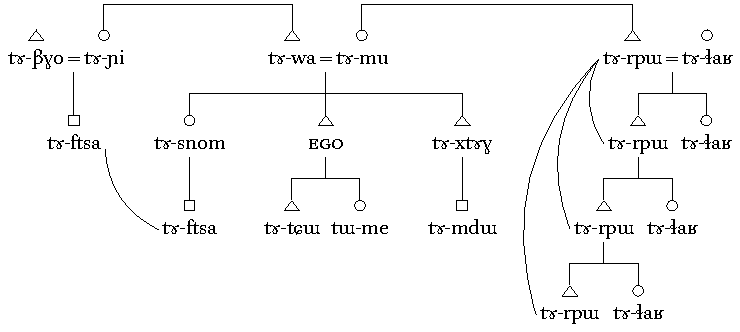
\includegraphics[width=\textwidth]{kinship-japhug-1.pdf}
\end{figure}
 
These \textit{skewing} rules\footnote{ \citet[357]{lounsbury64crow} defines this term as a `formal equivalence, in specific contexts, between kins of different generations'. } are reciprocal of each other.  They can be formally written as (\ref{ex:FZS.ZS}) and (\ref{ex:MBS.MB}) in Lounsbury's (\citeyear{lounsbury64crow}) fashion. \footnote{The rules (\ref{ex:FZS.ZS}) and (\ref{ex:MBS.MB}) are close to Lounsbury's (\citeyear[359]{lounsbury64crow}) `Omaha type I', but slightly less general. }
 
\begin{exe}
\ex 
\begin{xlist}
\ex \label{ex:FZS.ZS}
\glt \textbf{Skewing rule} 1: FZCh \fl{} ZCh
\ex \label{ex:MBS.MB}
\glt Corollaries:  MBS \fl{} MB; MBD \fl{} MZ
\end{xlist}
\end{exe}

Moreover, the fact that the children of one paternal aunt's children are also identified with the sister's children (§\ref{sec:MBCh.FZCh.Ch}) implies the rule in (\ref{ex:FZChCh.ZS}) and its reciprocal (\ref{ex:MMBS.MB}), explicitly stated by \iai{Tshendzin} in (\ref{ex:MMBCh.FMBCh}).

\begin{exe}
\ex \label{ex:MMBCh.FMBCh}
\gll nɤ-ɲi ɣɯ ɯ-ɣe kɯ tɕe tɕe, nɤj nɤ-ɕki ``a-rpɯ" tu-ti kɯ-ra ɕti. \\
\textsc{2sg}.\textsc{poss}-FZ \textsc{gen} \textsc{3sg}.\textsc{poss}-grandchild \textsc{erg} \textsc{lnk} \textsc{lnk} \textsc{2sg} \textsc{2sg}.\textsc{poss}-\textsc{dat} \textsc{1sg}.\textsc{poss}-MB \textsc{ipfv}-say \textsc{inf}:\textsc{stat}-be.needed be.\textsc{aff}:\textsc{fact} \\
\glt `Your father's sister's grandchildren have to call you `my mother's brother'.' (elicitation 2019-11-30)
\end{exe}

\begin{exe}
\ex 
\begin{xlist}
\ex \label{ex:FZChCh.ZS}
\glt \textbf{Skewing rule} 2: FZChCh \fl{} FZCh \fl{} ZCh
\ex \label{ex:MMBS.MB}
\glt Corollaries:  (F|M)MBS \fl{} MB; (F|M)MBD \fl{} MZ
\end{xlist}
\end{exe}
 
The rules (\ref{ex:FZS.ZS}), (\ref{ex:MBS.MB}), (\ref{ex:FZChCh.ZS}), (\ref{ex:MMBS.MB}) are described by \iai{Tshendzin} as being recursive, implying the theoretical equivalences in (\ref{ex:kinship.recursive}). Although a considerable amount of genealogies would be needed to confirm whether the system indeed works in the way predicted in (\ref{ex:kinship.recursive}), an anecdote discussed in §\ref{sec:MBChCh.Dpalcan} confirms the reality of the equivalence MMMBSSSS = MB.
  
 \begin{exe}
 \ex \label{ex:kinship.recursive}
\begin{xlist}
\ex \label{ex:FFFFZCh}
\glt ZCh = (F)*ZCh(Ch)*
\ex \label{ex:MBSSSS}
\glt MB = (F|M)*MB(S)*S
 \ex \label{ex:MBSSSD}
\glt MZ = (F|M)*MB(S)*D
\end{xlist}
\end{exe}

Another skewing rule is observed in the case of female \textsc{ego}:  \textsuperscript{♀}BS are called with the relative age sibling terms (§\ref{sec:nephews}), though this skewing is only partial, since they respond using the dedicated term \forme{tɤ-ɲi} for FZ (§\ref{sec:uncle.aunt}).

Finally, another skewing rule (\ref{ex:MZChCh.skewing}) appears with maternal parallel cousins (§\ref{sec:FBCh.MZCh.Ch}).

\begin{exe}
\ex 
\begin{xlist}
\ex \label{ex:MZChCh.skewing}
\glt \textbf{Skewing rule} 3: MZChCh \fl{} MZCh
\ex \label{ex:MMZCh.skewing}
\glt Corollary:  (F|M)MZCh \fl{} MZCh
\end{xlist}
\end{exe}

If the rules (\ref{ex:MZChCh.skewing}) and (\ref{ex:MMZCh.skewing}) are also recursive, the formal equivalence (\ref{ex:MMMMMZChChChCh}) is implied. Data is lacking to ascertain whether this theoretical possibility is verified, but §\ref{sec:FMZCh.Tshendzin} discusses a case in these lines. In this system, unlike in that described by \citet[361]{lounsbury64crow}, the MMZCh are not equated with the MB and MZ (due to absence of the merging rules MZS \fl{} B and MZD \fl{} Z), but rather with the MZCh. 

 \begin{exe}
\ex \label{ex:MMMMMZChChChCh}
\glt MZCh = (F|M)*MZCh(Ch)*
\end{exe}

However, it appears to be possible to alternatively use the term \forme{tɤ-ftsa} `ZS' for MZChCh. The implication of this rule for the whole system are not considered here until further data are available.

The terminological identification of paternal parallel cousins with siblings (§\ref{sec:ego.parallel.cousins}) defines the following merging rule (\ref{ex:FBS.B.FBD.Z}).

\begin{exe}
\ex \label{ex:FBS.B.FBD.Z}
\glt \textbf{Merging rules}: FBS \fl{} B; FBD \fl{} Z
\end{exe}

Unlike the Omaha systems described in \citet[360]{lounsbury64crow}, the merging rule (\ref{ex:FBS.B.FBD.Z}) does not concern maternal parallel cousins (§\ref{sec:ego.parallel.cousins}). It implies the equivalences MFBS = MB, MFBD = MZ, FFBS = FB and FFBD = FZ, and more generally (\ref{ex:kinship.recursive2}), in combination with the skewing rules in (\ref{ex:kinship.recursive}) above.

 \begin{exe}
 \ex \label{ex:kinship.recursive2}
\begin{xlist}
\ex  
\glt MB = (F|M)*MFB(S)*S
\ex  
\glt MZ = (F|M)*MFB(S)*D
\ex  
\glt FB = (F)$^n$FB(S)$^n_{n\geqslant 1}$
\ex  
\glt FZ = (F)$^n$FB(S)$^{n-1}$D$_{n\geqslant 1}$
\end{xlist}
\end{exe}
%\textsuperscript{♂}\textsuperscript{♀}

Some uncertainty remains in parts of the system. In particular, the status of the MBDCh (and its reciprocal MFZCh) is unclear. In theory, given the MBD \fl{} MZ rule (\ref{ex:MMBS.MB}), one would expect that MBDCh = MZCh (\forme{tɤ-mɤtsa}), and likewise that the MFZCh = MZCh (due to the reciprocal rule \ref{ex:FFFFZCh}). However, at the moment of writing I could not confirm whether this is true or not.
 
%\citet[359]{lounsbury64crow} proposes slightly more general formal rules for his `Omaha type I', rewritten in (\ref{ex:FZX.ZX}) and (\ref{ex:XBS.XB}) (X stands for any relative; the notation in slightly altered to fit the system used in this chapter).  
% 
%\begin{exe}
%\ex 
%\begin{xlist}
%\ex \label{ex:FZX.ZX}
%\glt \textbf{Skewing rule}: FZX \fl{} ZX
%\ex \label{ex:XBS.XB}
%\glt Corollaries:  X\textsuperscript{♀}BS \fl{} X\textsuperscript{♀}B; X\textsuperscript{♀}BD \fl{} X\textsuperscript{♀}Z
%\end{xlist}
%\end{exe}
% 
%For this formulation to be compatible with the Japhug system,  affines have to be excluded, since they are not concerned by the skewing rule. Otherwise,  FZH would be equivalent to ZH and WBS to WB. In fact, FZH is called using the FB term (see \tabref{tab:uncle.aunt}, §\ref{sec:uncle.aunt}), and ZH with the relative age sibling terms (§\ref{sec:siblings.age}).  

The Japhug system shows prototypical Omaha characteristics, in particular the basic skewing rules  (\ref{ex:FZS.ZS}) and (\ref{ex:MBS.MB}), and the identification of paternal parallel cousins with siblings (\ref{ex:FBS.B.FBD.Z}). It differs from prototypical Omaha systems described in the literature in lacking an Iroquois pattern identifying parallel uncles and aunts with parents (FB \fl{} F, MZ \fl{} M, \citealt[34]{trautmann12crossness}), maternal parallel cousins with siblings (MZS \fl{} B, MZD \fl{} Z), and the fact that preferred marriage is with maternal parallel cousins (§\ref{sec:marriage.rules}) rather than with cross-cousins (\citealt[41]{trautmann12crossness}).
 

 \subsection{Cross-cousin lineages} \label{sec:MBChCh.Dpalcan}
  \is{Omaha skewing rule}
A logical consequence of the recursivity of the skewing rule (\ref{ex:kinship.recursive}, §\ref{sec:skewing.merging}), as they are described by \iai{Tshendzin} (§\ref{sec:MBCh.FZCh.Ch}) is that a considerable divergence between biological age and age rank will occur in some cases. While a full investigation of genealogies is necessary to verify this implication (an endeavour that goes beyond the scope of this grammar), an  anecdote reported by two witnesses suggests that this indeed used to be the case in the traditional society.

In (\ref{ex:aftsa.beifen}), a man born in the 1950s reports his experience with the skewing rule: one of his great-grandmother (either MMM or MMMM, I could not ascertain) came from the village of Tshapa (with irregular orientation \textsc{westwards}, opposite of the geographical reality, §\ref{sec:local.toponyms.orientation}), where most inhabitants are from the lineage of her brother.

 \begin{exe}
\ex \label{ex:aftsa.beifen}
\gll  iʑo ji-wi nɯnɯ tsʰapa nɯ-kɯ-ɣe pjɤ-ŋu. (...)   aʑo tɤ-nɯkoŋtso-a ɯ-qʰu tɕe, tsʰapa ju-ɕe-a tɕe, tsʰapa nɯ ji-kɯmdza ʁɟa ɲɯ-ŋu tɕe, (...) tɕe a-rpɯ a-ɬaʁ ntsɯ tu-kɯ-ti ɲɯ-ra ma nɯ-<beifen> ɲɯ-mbro, (...)   tɤ-pɤtso kɯ-xtɕɯ\redp{}xtɕi ra kɯ nɯ a-pʰe ``a-ftsa a-ftsa" tu-ti-nɯ, ``a-rpɯ a-ɬaʁ" kɤ-ti ɲɯ-ra, tɕendɤre tu-ti-a kɯ-zgɤt ɲɯ-ɕti ri nɯnɯ aʑo mɯ́j-nɤx-tʂaŋ-a   \\
\textsc{1pl} \textsc{1pl}.\textsc{poss}-grandmother \textsc{dem}  \textsc{topo} \textsc{aor}:\textsc{west}-\textsc{sbj}:\textsc{pcp}-come[II] \textsc{ifr}.\textsc{ipfv}-be { } \textsc{1sg} \textsc{aor}-work-\textsc{1sg} \textsc{3sg}.\textsc{poss}-after \textsc{lnk}  \textsc{topo} \textsc{ipfv}-go-\textsc{1sg} \textsc{lnk}  \textsc{topo} \textsc{dem} \textsc{1pl}.\textsc{poss}-relative completely \textsc{sens}-be \textsc{lnk} { } \textsc{lnk} \textsc{1sg}.\textsc{poss}-MB \textsc{1sg}.\textsc{poss}-MZ always \textsc{ipfv}-\textsc{genr}-say \textsc{sens}-be.needed \textsc{lnk} \textsc{3pl}.\textsc{poss}-age.rank \textsc{sens}-be.high {  } \textsc{indef}.\textsc{poss}-child \textsc{sbj}:\textsc{pcp}-\textsc{emph}\redp{}be.small \textsc{pl} \textsc{erg} \textsc{dem}  \textsc{1sg}.\textsc{poss}-\textsc{dat}  \textsc{1sg}.\textsc{poss}-ZCh  \textsc{1sg}.\textsc{poss}-ZCh \textsc{ipfv}-say-\textsc{pl}  \textsc{1sg}.\textsc{poss}-MB \textsc{1sg}.\textsc{poss}-MZ \textsc{inf}-say \textsc{sens}-be.needed \textsc{lnk} \textsc{ipfv}-say-\textsc{1sg} \textsc{inf}:\textsc{stat}-be.needed \textsc{sens}-be.\textsc{aff} \textsc{lnk} \textsc{dem} \textsc{1sg} \textsc{neg}:\textsc{sens}-\textsc{trop}-be.fair-\textsc{1sg} \\
\glt `[One of] our grandmothers was from Tshapa (...) After I started working, when I went to Tshapa, everybody there is a relative of ours, (...) I had to call all of them `my mother's brother, my mother's sister', because they are of higher \ch{辈分}{bèifen}{age rank}, (...) [even] small children called me `my sister's son', and I had to call them  `my mother's brother, my mother's sister'. Although this was what I had to say, I found it unfair.' (2010-06)
 \end{exe}
 
He thus had to call all the inhabitants of the village using the MB  and MZ  terms \forme{tɤ-rpɯ}  and \forme{tɤ-ɬaʁ}, even young children. This report suggests that the recursivity of the rules as described in (\ref{ex:kinship.recursive}) above is a reality: descendants of MMMB or MMMMB, even one or two generations below oneself, are still called MB and MZ. It also suggests that not only MBS*, but also MBDCh and their descendants might keep the privileged status (and thus not be equated with maternal parallel cousins MZCh as predicted in §\ref{sec:skewing.merging}), though this has to be tested with additional data.

\iai{Tshendzin} reports the same anecdote (\ref{ex:MMMMMBSSSSS}), and also indicates that the recursivity of the skewing rule is felt clumsy by younger speakers, who prefer to use terms for parallel uncles, aunts or siblings. This aspect of the Japhug languages is thus highly endangered.
 
 \begin{exe}
\ex \label{ex:MMMMMBSSSSS}
\gll  ɯ-wi ɣɯ ɯ-wi nɯnɯ tsʰapa nɯtɕu nɯ-kɯ-ɣe pjɤ-ŋu tɕe tɕe nɯ ɣɯ ɯ-wi ɣɯ ɯ-wɤmɯ nɯnɯ ɣɯ ɯ-rɟit ɣɯ ɯ-rɟit ɣɯ ɯ-rɟit ɣɯ ɯ-rɟit kɯ-fse nɯnɯra nɯ-ɕki tɕe tɕe ``a-rpɯ nɤ a-ɬaʁ" ntsɯ tu-ti pjɤ-ra. (...) tʰam tɕe nɯra stʰɯci ɯ-kɯ-ti maŋe, tɕe kɯ-xtɕi nɯra kɯnɤ ``a-ftsa" kɤ-ti ɲɯ-nɤzraʁ-nɯ qʰe ``a-βɣo" ra tu-nɯ-ti-nɯ,  ``a-pi" ra tu-nɯ-ti-nɯ. tɕe tʰam tu-otʂoʁloʁ ɕti. kɯɕɯŋgɯ a-pɯ-ŋu tɕe nɯ tu-kɯ-ti kɯ-ra pjɤ-ɕti nɤ. \\
  \textsc{3sg}.\textsc{poss}-grandmother \textsc{gen}   \textsc{3sg}.\textsc{poss}-grandmother \textsc{dem}   \textsc{topo} \textsc{dem}:\textsc{loc} \textsc{aor}:\textsc{west}-\textsc{sbj}:\textsc{pcp}-come[III] \textsc{ifr}.\textsc{ipfv}-be \textsc{lnk} \textsc{lnk} \textsc{dem} \textsc{gen} \textsc{3sg}.\textsc{poss}-grandmother \textsc{gen} \textsc{3sg}.\textsc{poss}-brother \textsc{dem} \textsc{gen} \textsc{3sg}.\textsc{poss}-offspring  \textsc{gen} \textsc{3sg}.\textsc{poss}-offspring  \textsc{gen} \textsc{3sg}.\textsc{poss}-offspring  \textsc{gen} \textsc{3sg}.\textsc{poss}-offspring \textsc{sbj}:\textsc{pcp}-be.like \textsc{dem}:\textsc{pl} \textsc{3pl}.\textsc{poss}-\textsc{dat} \textsc{loc} \textsc{lnk} \textsc{1sg}.\textsc{poss}-MB \textsc{add} \textsc{1sg}.\textsc{poss}-MZ always \textsc{ipfv}-say \textsc{ipfv}.\textsc{ifr}-be.needed {  } now \textsc{lnk} \textsc{dem}:\textsc{loc} so.much \textsc{3sg}.\textsc{poss}-\textsc{sbj}:\textsc{pcp}-say not.exist:\textsc{sens} \textsc{lnk} \textsc{sbj}:\textsc{pcp}-be.small \textsc{dem}:\textsc{pl} also \textsc{1sg}.\textsc{poss}-ZCh \textsc{inf}-say \textsc{sens}-be.ashamed-\textsc{pl} \textsc{lnk} \textsc{1sg}.\textsc{poss}-FB \textsc{pl} \textsc{ipfv}-\textsc{auto}-say-\textsc{pl} \textsc{1sg}.\textsc{poss}-elder.sibling \textsc{pl} \textsc{ipfv}-\textsc{auto}-say-\textsc{pl}  \textsc{lnk} now \textsc{ipfv}-be.mixed be.\textsc{aff}:\textsc{fact} in.former.days \textsc{irr}-\textsc{ipfv}-be \textsc{lnk} \textsc{dem} \textsc{ipfv}-\textsc{genr}-say \textsc{inf}:\textsc{stat}-be.needed \textsc{ifr}.\textsc{ipfv}-be \textsc{sfp} \\
 \glt `His grandmother's grandmother had come from Tshapa, and he had to call all of his grandmother's brother's children's children's children's children (etc) `my mother's brother, my mother's sister' (including small children)'. (...) Now no one says this any more, the young ones are ashamed of calling [elders] `my sister's child' and instead say `my father's brother' or `my elder sibling'. Now it is all mixed up, but in former times, one had to speak like that.' (140425 kWmdza07) \japhdoi{0003791}
 \end{exe}
 
 \subsection{Maternal parallel cousin lineages} \label{sec:FMZCh.Tshendzin}
 The reliability of the skewing rule (\ref{ex:MZChCh.skewing}) concerning maternal parallel cousins is confirmed by one particular case, in which a lady addressed her mother-in-law by the term \forme{tɤ-mɤtsa} `MZCh' (who answered using the same term, §\ref{sec:ego.parallel.cousins}). When I asked her whether they were actual maternal parallel cousins (children of two sisters, MZCh), she answered that she used this term because her father himself called her mother-in-law (and her mother-in-law's mother) \forme{tɤ-mɤtsa}, though they were not themselves true first cousins, the eventual consanguine relationship going back several generations. She also specified that she called her husband \forme{tɤ-mɤtsa} before marrying him (§\ref{sec:marriage.rules}). 
 
This case suggests that the reciprocal \forme{tɤ-mɤtsa} `maternal parallel cousin' relationship remains regardless of the number of generations in each lineages (as formalized in \ref {ex:MMMMMZChChChCh} above).

\subsection{Application} \label{sec:cousins.once.rmoved}
As an illustration of the rules established in the previous sections, \tabref{sec:cousin.once} summarizes the theoretical possibilities for first and second cousins \textit{once removed}, including the main points of uncertainty in grey shading. The equivalences are given below each term in brackets, referring to the equivalent focal kin (\tabref{tab:focal.kin}); for instance (=ZCh) should be read `called like the ZCh' (\forme{tɤ-ftsa}, §\ref{sec:nephews}). 

\begin{table}
\caption{Focal kin terms } \label{tab:focal.kin}
\begin{tabular}{lllll}
\lsptoprule
 Kin & term & Reciprocal & term \\
\midrule
M& \forme{tɤ-mu} & \textsuperscript{♀}S/\textsuperscript{♀}D &\forme{tɤ-tɕɯ}/\forme{tɯ-me} \\
F &\forme{tɤ-wa} & \textsuperscript{♂}S/\textsuperscript{♂}D &\forme{tɤ-tɕɯ}/\forme{tɯ-me} \\
\midrule
MB  &  \forme{tɤ-rpɯ} & \textsuperscript{♂}ZCh &\forme{tɤ-ftsa} \\
MZ &\forme{tɤ-ɬaʁ} & \textsuperscript{♀}ZCh &\forme{tɤ-ftsa} \\
\midrule
FB  & \forme{tɤ-βɣo} & \textsuperscript{♂}BCh &\forme{tɤ-mdɯ} \\
FZ & \forme{tɤ-ɲi} & \textsuperscript{♂}BCh=yB|Z &\forme{ta-ʁi} \\
\midrule
MZCh & \forme{tɤ-mɤtsa} & = \\
\midrule
eB|Z &\forme{tɤ-pi} & yB|Z &\forme{ta-ʁi} \\
\midrule
\textsuperscript{♂}Z& \forme{tɤ-snom} & \textsuperscript{♀}B \forme{tɤ-wɤmɯ} \\
\textsuperscript{♂}B& \forme{tɤ-xtɤɣ} & =  \\
\textsuperscript{♀}Z& \forme{tɤ-sqʰaj} & = \\
\lspbottomrule
\end{tabular}
\end{table}

The reciprocal terms can be rechecked using the inversion table \ref{tab:kinship.reciprocal} above.

It is difficult to be fully certain of the reliability of these extrapolations without an in-depth study of genealogies. This Table provides a framework for future research on kinship systems in Japhug and Gyalrong-speaking areas. 

\begin{table}
\caption{First and second cousins once removed (hypothetical)} \label{sec:cousin.once}
\begin{tabular}{lllll}
\lsptoprule
First cousin  & Reciprocal & Second cousin &  Reciprocal \\ 
\midrule
FFBS  & \textsuperscript{♂}FBSCh  & FFBSCh  & FFBSCh \\
(=FB)& (=\textsuperscript{♂}BCh) &(= FBCh=B|Z)& (=B|Z) \\
\midrule
FFBD & \textsuperscript{♀}FBSCh& FFBDCh  & MFBSCh  \\
 (=FZ) & (=\textsuperscript{♀}BS=yB|Z) &  (= FZCh=ZCh) &  (=MBCh=MB|Z) \\
\midrule
FFZCh   & MBSS  & FFZChCh   & (F|M)MBSS   \\
(=ZCh) &  (=MB) &  (=ZCh) & (=MB) \\
\midrule
FMBS  & \textsuperscript{♂}FZSCh   & FMBSCh  &  FFZSCh  \\
 (=MB) & (=ZCh) &  (=MB) &   (=ZCh) \\
 \midrule
FMBD   & \textsuperscript{♀}FZSCh   & FMBDCh  &  MFZSCh  \\
 (=MZ) &  (=ZCh) &  (=FMZCh=MZCh?)\grise{} &   (=MZCh?) \grise{}\\
\midrule
FMZCh   & MZDS   & FMZChCh  &  (F|M)MZDS  \\
 (=MZCh?)\grise{} &  (=MZCh?)\grise{}&  (=MZCh?)\grise{}&  (=MZCh?)\grise{} \\
\midrule
MFBS  & \textsuperscript{♂}FBDCh &MFBSCh & FFBDCh  \\
 (=MB) & (=FZCh=ZCh) & (=MB|Z)&  (=FFZCh=ZCh) \\
 \midrule
MFBD & \textsuperscript{♀}FBDCh &MFBDCh & MFBDCh  \\
 (=MZ) & (=FZCh=ZCh) & (=MZCh?)\grise{}&  (=MZCh?)\grise{} \\
\midrule
MFZCh  &  MBDCh &MFZChCh & (F|M)MBDCh  \\
 (=MZCh?)\grise{} &  (=MZCh?)\grise{}&  (=MZCh?)\grise{}&  (=MZCh?)\grise{} \\
 \midrule
 MMBS  & \textsuperscript{♂}FZDCh &MMBSCh & FFZDCh  \\
 (=MB) & (=ZCh) & (=MB|Z)&  (=ZCh) \\
  \midrule
  MMBD  & \textsuperscript{♀}FZDCh &MMBDCh & MFZDCh  \\
 (=MMZ=MZ) & (=ZCh) & (=MZCh?)\grise{} &  (=MZCh?) \grise{} \\
   \midrule
  MMZCh  & MZDCh &MMZChCh & (F|M)MZDCh  \\
   (=MZCh) &  (=MZCh) &  (=MZCh?) \grise{}&  (=MZCh?)\grise{} \\
\lspbottomrule
\end{tabular}
\end{table}
 